\chapter{Аналитический раздел}

\section{Описание предметной области}
Тело вращения —-- это объект, образованный вращением плоской линии (образующей) вокруг фиксированной оси (направляющей). Таким образом, любая точка образующей описывает окружность, центр которой лежит на оси вращения, а само тело получается симметричным относительно этой оси~\cite{Тела_вращения}.

\section{Методы задания кривой}
Образующая задается как плоская кривая, поэтому необходимо рассмотреть методы задания кривых линий:
\subsection{Полиномиальные кривые}
Полиномиальные кривые задаются аналитическими уравнениями вида:
\begin{equation}
    y = a_nx^n + a_{n-1}x^{n-1} + ... + a_1x + a_0,
\end{equation}
где $n$ --- степень полинома, а $a_i$ --- его коэффициенты. Метод задания кривой заключается в определении коэффициентов полинома $a_i$. Для этого для заданного количества точек $k$ необходимо решить систему из $k$ уравнений:
\begin{equation}
    \begin{cases}
    y_1 = a_{k-1}x_1^{k-1} + a_{k-2}x_1^{k-2} + ... + a_0 \\
    y_2 = a_{k-1}x_2^{k-1} + a_{k-2}x_2^{k-2} + ... + a_0 \\
    \vdots	\\
    y_k = a_{k-1}x_k^{k-1} + a_{k-2}x_k^{k-2} + ... + a_0 \\
    \end{cases}.
\end{equation}
После нахождения коэффициентов уравнения можно вычислить значение кривой для любого $x$ в заданном диапазоне. Однако не всегда получается найти точное решение системы, также при высоких степенях полинома может возникнуть эффект Рунге, из-за которого кривая будет задана отличным от ожидаемого образом, с выраженными осцилляциями~\cite{Рунге}.

\subsection{Кубические сплайны}
Кубические сплайны --- это составные полиномиальные кривые третьей степени, обеспечивающие гладкость соединения сегментов. Каждый сегмент сплайна на интервале $[x_i, x_{i+1}]$ описывается уравнением:
\begin{equation}
    S_i(x) = a_ix^3 + b_ix_2 + c_ix + d_i,
\end{equation}
где $a_i, b_i, c_i, d_i$ --- коэффициенты, определяемые для каждого сегмента. Для задания кривой вычисляются коэффициенты для каждого из сегментов кривой путем решения системы уравнений, которая учитывает непрерывность на стыках сегментов функции, первой производной и второй производной:
\begin{equation}
    \begin{cases}
    S_i(x_{i+1}) = S_{i+1}(x_{i+1}) \\
    S_i'(x_{i+1}) = S_{i+1}'(x_{i+1}) \\
    S_i''(x_{i+1}) = S_{i+1}''(x_{i+1}) \\
    \end{cases}.
\end{equation}
После вычисления коэффициентов кривая задается как последовательность сегментов.

\subsection{Кривая Безье}
Кривая Безье определяется контрольными точками $P_0, P_1,...,P_n$. Эти точки задают форму кривой, но сама кривая не обязательно будет проходить через все точки, кроме крайних. 

Для построения кривой используется алгоритм де Кастельжо~\cite{кривые_безье}. Для каждого значения параметра $t \in [0, 1]$, итеративно вычисляются новые точки $P_{i,j}$ по формуле:
\begin{equation}
    P_{i,j} = (1 -t)P_{i-1,j} + tP_{i,j+1},
\end{equation}
где $P_{i-1,j}, P_{i,j-1}$ -- соседние точки на предыдущем уровне итерации, $t$ --- параметр интерполяции, определяющий положение точки между ними. Процесс начинается с заданного набора контрольных точек (нулевой уровень). На каждом последующем уровне число точек уменьшается, так как каждая новая точка вычисляется как интерполяция двух точек предыдущего уровня. Алгоритм продолжается до тех пор, пока не останется единственная точка, которая и будет являться точкой кривой для данного значения параметра $t$. 

Использование кривых Безье позволяет задавать кривые различных форм, которые можно легко построить на плоскости по заданным точкам с помощью алгоритма де Кастельжо.

\subsection{Выбор метода задания кривой}
В качестве метода задания кривых были выбраны кривые Безье, так как с их помощью можно задавать кривые различных форм, а с помощью алгоритма де Кастельжо их легко строить на плоскости без необходимости производить сложные вычисления. 

\section{Алгоритмы построения тела вращения}
Рассмотрим несколько существующих алгоритмов построения тела вращения:
\begin{itemize}
    \item[---] \textbf{Построение при дискретном представлении тела.} При дискретном представлении тело вращения задается множеством примитивов (полигонов), которые являются математическим приближением тела. Образующая разбивается на множество точек, каждая точка вращается вокруг выбранной направляющей. Полученные точки являются вершинами полигонов, которые задают тело;
    \item[---] \textbf{Построение при аналитическом представлении}. При аналитическом представлении тело вращения описывается с использованием параметрических уравнений, которые выражают положение каждой точки поверхности через параметры. Образующая задается аналитической функцией $f(x)$, описывающей ее форму. Для построения тела вращения вычисляются координаты точек поверхности путем вращения образующей вокруг оси с использованием параметрических формул;
    \item[---] \textbf{Построение при произвольной направляющей.} Если направляющая задается как произвольная кривая, то необходимо рассмотреть движение образующей вдоль этой прямой в пространстве. Образующая сдвигается и вращается вдоль направляющей, формируя тело вращения. 
\end{itemize}

\subsection{Выбор алгоритма построения тела вращения}
Для визуализации тел вращения в данной работе был выбран алгоритм построения при дискретном представлении тела. Поскольку направляющая задается одной из координатных осей, отсутствует необходимость учитывать сложные преобразования, связанные с произвольной направляющей. Кроме того, данный подход предпочтителен по сравнению с алгоритмом аналитического построения, так как он обеспечивает большую гибкость в представлении сложных форм. Алгоритм дискретного представления позволяет работать с любыми кривыми, заданными конечным набором точек, что упрощает реализацию и делает его более универсальным.

\section{Алгоритмы удаления невидимых линий}
Для построения реалистичного трехмерного изображения необходимо определить, какие линии или поверхности объектов видимы для наблюдателя, а какие нет.

Алгоритмы удаления невидимых линий и поверхностей служат для определения линий, поверхностей или объемов, которые видимы или невидимы для наблюдателя, находящегося в заданной точке пространства.

\subsection{Алгоритм Варнока}
Основная идея алгоритма Варнока заключается в решении вопроса: что нужно отображать в каждом конкретном окне изображения. Изначально окно охватывает весь экран. Если невозможно сразу определить, что отображать, окно делится на четыре части. В результате получается 4 окна меньших размеров. Если и для них невозможно дать точный ответ, процесс деления продолжается до тех пор, пока каждое окно не станет достаточно малым, чтобы дать однозначный ответ, или пока размер окна не достигнет одного пикселя~\cite{Varnok_alg}.

На рисунке~\ref{fig:varnok_ex} показан пример разбиения по алгоритму Варнока.
\begin{figure}[H]
	\centering
	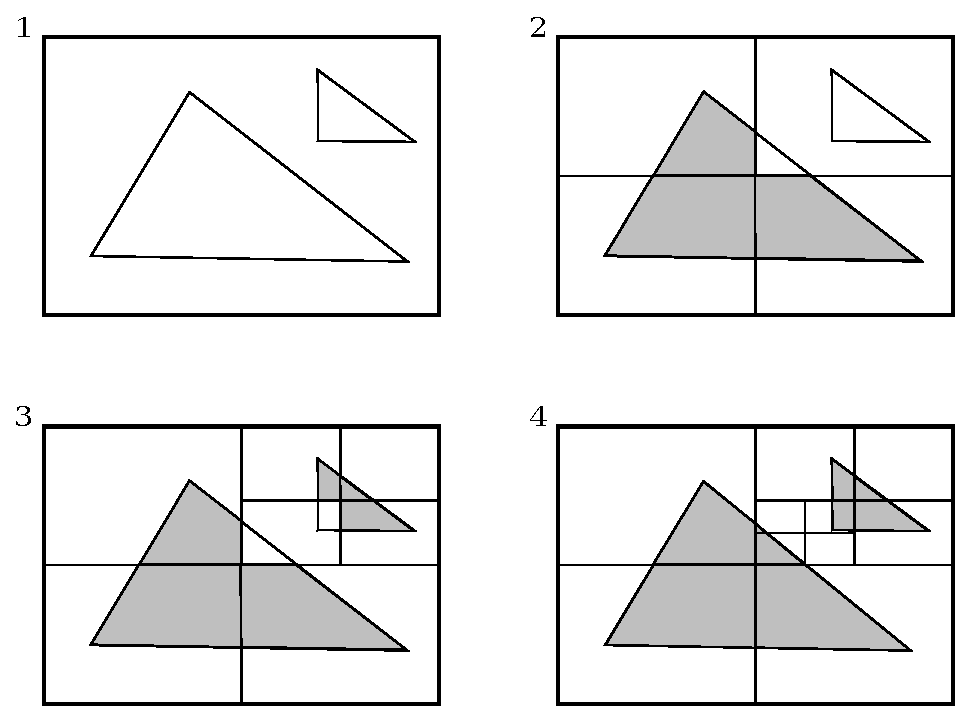
\includegraphics[scale=0.6]{img/Varnok_alg.eps}
	\caption{Пример разбиения алгоритмом Варнока}
	\label{fig:varnok_ex}
\end{figure}

Из недостатков алгоритма можно отметить необходимость производить большое количество разбиений при визуализации сложной сцены.


\subsection{Алгоритм Z-буфера}
Алгоритм Z-буфера решает задачу скрытых поверхностей, используя два буфера: буфер кадра, который хранит информацию о цвете и яркости пикселей, и Z-буфер, фиксирующий координаты глубины. Процесс начинается с инициализации Z-буфера максимальными значениями глубины, а буфера кадра --- значениями фона. Для каждого многоугольника сцены его пиксели сравниваются с пикселями в Z-буфере, и если значение глубины для текущего пикселя меньше соответствующего значения в Z-буфере, то происходит обновление как в буфере кадра, так и в Z-буфере.

Этот метод прост и эффективен для работы с произвольными сценами, но требует значительных объемов памяти для хранения глубины каждого пикселя. Также он имеет ограничения при работе с прозрачными объектами и сглаживании лестничного эффекта на границах многоугольников.

\subsection{Алгоритм прямой трассировки лучей}
Алгоритм прямой трассировки лучей заключается в том, что лучи света испускаются от источника и распространяются по сцене, взаимодействуя с объектами. Когда свет достигает поверхности объекта, он может отражаться, поглощаться или преломляться в зависимости от свойств материала. Для каждого такого взаимодействия необходимо просчитать, куда направляется луч, и что происходит с его интенсивностью и цветом. Задача алгоритма —-- вычислить траекторию света от источника до наблюдателя, моделируя эффекты отражения, преломления и рассеивания, что позволяет учесть такие явления, как тени, отражения и прохождение света через полупрозрачные объекты.

Основная сложность прямой трассировки заключается в том, что лишь небольшая часть лучей, испущенных от источников света, достигает поверхности камеры или экрана, что делает метод вычислительно затратным. Этот алгоритм требует большого количества лучей для получения реалистичного изображения, что значительно увеличивает время рендеринга сложных сцен~\cite{ray_tracing}.

\subsection{Алгоритм обратной трассировки лучей}
Алгоритм обратной трассировки лучей работает по принципу, противоположному прямой трассировке. Вместо того, чтобы испускать лучи от источников света, алгоритм начинает с наблюдателя. Каждый луч проходит через пиксели изображения и пересекают объекты в сцене. Когда луч достигает поверхности объекта, он может отразиться, переломиться или поглотиться. Отраженные и преломленные лучи продолжают свое движение по сцене, пока не встретят другие объекты или не будут отброшены. Для расчета эффектов освещения проводятся вторичные лучи от точек пересечения до всех источников света. Если вторичный луч пересекается с непрозрачным телом, то точка, из который вторичный луч был выпущен, находится в тени. 

Этот метод более эффективен, поскольку вычисления ведутся только для тех лучей, которые попадают в камеру, что позволяет существенно сократить число обрабатываемых лучей по сравнению с прямой трассировкой. Кроме того, обратная трассировка лучей может точно учитывать такие эффекты, как отражения, преломления и тени, делая изображение более реалистичным. Однако, несмотря на свою эффективность по сравнению с прямой трассировкой, обратная трассировка все же требует значительных вычислительных ресурсов для сложных сцен с большим количеством объектов.

Для оптимизации количества вычислений можно поместить объект в выпуклую оболочку: сферическую или в форме параллелепипеда. Таким образом, если луч не пересекает оболочку тела, то он не пересекает и само тело, значит не нужно искать пересечение луча и тела.

Визуализация работы алгоритма обратной трассировки лучей приведена на рисунке~\ref{fig:raytrassing}.

\begin{figure}[H]
	\centering
	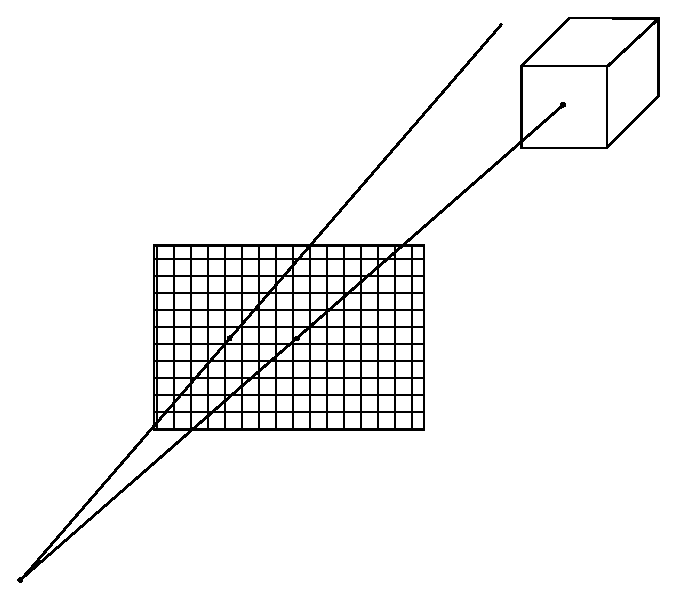
\includegraphics[scale=0.6]{img/raytrassing.eps}
	\caption{Пример трассировки лучей}
	\label{fig:raytrassing}
\end{figure}

\subsection{Выбор алгоритма удаления невидимых линий}
В данной работе для удаления невидимых линий был выбран алгоритм Z-буфера благодаря его простоте и скорости работы, что важно для взаимодействия с полученным телом в реальном времени с минимальными задержками.

\section{Алгоритмы закрашивания}
Существует несколько алгоритмов закрашивания:
\begin{itemize}
    \item[---] \textbf{Однотонная закраска.} Этот метод довольно прост в своей реализации. Для каждой грани объекта вычисляется уровень освещенности, который применяется одинаково ко всей поверхности грани. Это обеспечивает быструю обработку, однако изображение выглядит плоским, так как не учитывается плавный переход интенсивности света между различными частями объекта;
    \item[---] \textbf{Закраска по Гуро.} В данном методе интенсивность света вычисляется для каждой вершины грани, а затем интерполируется. Этот метод позволяет получить гораздо более визуально-приятное изображение. Это позволяет сгладить переходы между различными частями поверхности, что улучшает визуальное восприятие объекта. Однако при низком уровне детализации блики могут быть смазанными, так как интенсивность света не пересчитывается для каждой точки поверхности, а лишь интерполируется;
    \item[---] \textbf{Закраска по Фонгу.} В этом методе используется интерполяция вектора нормали к поверхности вместо интерполяции интенсивности. Интерполяция выполняется между начальной и конечной нормалями, которые сами тоже являются результатом интерполяции вдоль ребер многоугольника между нормалями в вершинах. Данный метод требует гораздо большего количества вычисление, чем метод закраски по Гуро или метод однотонной закраски, но дает значительно лучшие результаты, а также позволяет применять методы рельефного текстурирования для визуализации неровностей~\cite{Затенение_и_освещение}.
\end{itemize}


В методах Гуро и Фонга необходимо рассчитывать значение нормали в вершинах многогранника. Нормаль в точке вычисляется путем путем усреднения нормали по всем полигональным граням, которым принадлежит вершина:
\begin{equation}
    \vec{N} = \frac{\displaystyle\sum_{i=1}^n \vec{N_i}}{n}.
\end{equation}

\subsection{Выбор алгоритма закрашивания}
В качестве алгоритма закрашивания был выбран алгоритм закраски по Фонгу, так как данный алгоритм позволяет максимально точно передать освещение благодаря детальной интерполяции нормалей на поверхности. Кроме того, этот метод идеально подходит для реализации рельефного текстурирования.

\section{Анализ моделей освещения}
Существует две модели освещения: локальная и глобальная. Локальная модель не рассматривает процессы светового взаимодействия объектов сцены между собой, рассчитывает освещенность только самих объектов. Глобальная модель рассматривает трехмерную сцену, как единую систему и описывает освещение с учетом взаимного влияния объектов.
Для поставленной задачи лучше подходит локальная модель освещения, так как она является более быстродействующей. Также в сцене отсутствуют объекты, обладающие зеркальными или преломляющими свойствами, поэтому использование более качественной глобальной модели не требуется.
Рассмотри наиболее популярные локальные модели освещения.

\subsection{Модель Ламберта}
Модель Ламберта моделирует идеальное диффузное освещение~\cite{Освещение}. Считается, что свет при попадании на поверхность рассеивается равномерно во все стороны. При расчете такого освещения учитывается только ориентация поверхности (нормаль) и направление на источник света. 
Рассеянную составляющую можно рассчитать по формуле~\ref{eq:Labert}:
\begin{equation}
    \label{eq:Labert}
    I_d = k_d \cdot \cos(\vec{L},\vec{N}) \cdot i_d,
\end{equation}
где $I_d$ - рассеянная составляющая освещенности в точке, $k_d$ - свойство материала воспринимать рассеянное освещение, $i_d$ - мощность рассеянного освещения, $L$ - направление из точки на источник, $N$ - вектор нормали в точке.

\subsection{Модель Фонга}
Модель Фонга –-- классическая модель освещения. Модель представляет собой комбинацию диффузной составляющей (модели Ламберта) и зеркальной составляющей и работает таким образом, что кроме равномерного освещения на материале может еще появляться блик~\cite{Освещение}. Местонахождение блика на объекте, освещенном по модели Фонга, определяется из закона равенства углов падения и отражения.

Падающий и отраженный лучи лежат в одной плоскости с нормалью к отражающей поверхности в точке падения, и эта нормаль делит угол между лучами на две равные части. Т.о. отраженная составляющая освещенности в точке зависит от того, насколько близки направления на наблюдателя и отраженного луча. Это можно выразить следующей формулой \ref{eq:Fong}:
\begin{equation}
    \label{eq:Fong}
    I_s = k_s \cdot \cos^\alpha(\vec{R}, \vec{V}) \cdot i_s,
\end{equation}
где $I_s$ - зеркальная составляющая освещенности в точке, $k_s$ - коэффициент зеркального отражения, $i_s$ - мощность зеркального освещения, $R$ - направление отраженного луча, $V$ - направление на наблюдателя, $\alpha$ - коэффициент блеска, свойство материала.

\subsection{Выбор модели освещения}
Так как сцена не предполагает наличия на ней зеркальных объектов, в данной курсовой работе используется модель освещения Ламберта. Модель обеспечивает приемлемое качество освещения, легко реализуется и интегрируется с закраской по Фонгу, а также наименее требовательна к вычислительным ресурсам.

\section{Анализ алгоритмов визуализации неровностей}
Существует несколько алгоритмов рельефного текстурирование:
\begin{itemize}
    \item[---] \textbf{Bump mapping.} Этот метод создает иллюзию рельефа на поверхности без изменения ее геометрии. Bump mapping использует карту высот, где каждый пиксель задает отклонение нормали поверхности. На основе этих нормалей пересчитываются эффекты освещения, что создает ощущение шероховатости~\cite{Текстурирование};
    \item[---] \textbf{Normal mapping.} Метод является развитием bump mapping и моделирует рельеф точнее за счет использования карты нормалей. В normal mapping для каждой точки поверхности хранятся три значения, соответствующие координатам вектора нормали, что дает более точные результаты при расчете освещения. Данный метод также не изменяет геометрию объекта, а лишь корректирует его освещенность~\cite{mapping};
    \item[---] \textbf{Parallax mapping.} Этот метод создает иллюзию глубины на поверхности, изменяя текстурные координаты в зависимости от угла зрения наблюдателя. Parallax mapping использует карту высот, где значения представляют относительные изменения высоты. На основе этой карты текстурные координаты смещаются, чтобы имитировать перспективу и визуализировать рельеф. Метод не изменяет геометрию объекта и используется для повышения реализма текстур при низких вычислительных затратах;
    \item[---] \textbf{Displacement mapping.} Этот метод физически изменяет геометрию объекта, преобразуя его поверхность в соответствии с картой высот. Каждая вершина модели смещается вдоль нормали поверхности на величину, указанную в карте. Это позволяет создавать реалистичный рельеф с правильным взаимодействием света и теней. Метод требует значительных вычислительных ресурсов и применяется в задачах, где важен высокий уровень реализма.
\end{itemize}

\subsection{Выбор алгоритма визуализации неровностей}
В качестве алгоритма визуализации неровностей был выбран normal mapping, так как данный алгоритм позволяет получить реалистичное отображение мелких деталей поверхности без увеличения количества геометрических примитивов. 

\textbf{ВЫВОД}

В данном разделе был проведен анализ существующих алгоритмов построения построения изображения. Для задания кривой была выбрана кривая Безье. Для получения тела вращения был выбран алгоритм построения при дискретном представлении тела. Для построения реалистичного изображения были выбраны алгоритм Z-буфера, модель освещения Ламберта, закраска по Фонгу, normal mapping. 
